% !TEX program = pdflatex
\documentclass[aspectratio=169]{beamer}
\usetheme{Madrid}
\usecolortheme{default}
\usepackage{tikz}
\usepackage{amsmath}
\usepackage{amssymb}

% Custom colors
\definecolor{myblue}{RGB}{0,114,178}
\definecolor{myorange}{RGB}{230,159,0}
\definecolor{mygreen}{RGB}{0,158,115}
\definecolor{myred}{RGB}{213,94,0}
\definecolor{mypurple}{RGB}{204,121,167}
\definecolor{mybrown}{RGB}{240,228,66}
\definecolor{mygray}{RGB}{189,189,189}

% Set colors
\setbeamercolor{title}{fg=white,bg=myblue}
\setbeamercolor{frametitle}{fg=white,bg=myblue}
\setbeamercolor{section title}{fg=white,bg=myblue}
\setbeamercolor{subsection title}{fg=white,bg=myorange}
\setbeamercolor{item}{fg=myblue}
\setbeamercolor{subitem}{fg=myorange}

% Remove navigation symbols
\setbeamertemplate{navigation symbols}{}

% Title page
\title{Multivariable Functions}
\subtitle{Partial Derivatives and Second Order Partials}
\author{Differential Calculus}
\date{}

\begin{document}

\begin{frame}
\titlepage
\end{frame}

\begin{frame}{Outline}
\tableofcontents
\end{frame}

\section{Introduction to Multivariable Functions}

\begin{frame}{What are Multivariable Functions?}
\begin{itemize}
    \item Functions that depend on more than one variable
    \item Examples: $f(x,y) = x^2 + y^2$, $g(x,y,z) = xyz + \sin(x)$
    \item Input: multiple variables (e.g., $(x,y)$ or $(x,y,z)$)
    \item Output: single real number
    \item Visualized as surfaces in 3D space
\end{itemize}

\textbf{Key Differences from Single Variable Functions:}
\begin{itemize}
    \item Domain: subset of $\mathbb{R}^n$ (n-dimensional space)
    \item Range: subset of $\mathbb{R}$ (real numbers)
    \item More complex behavior and visualization
    \item Multiple ways to approach a point
\end{itemize}
\end{frame}

\begin{frame}{Examples of Multivariable Functions - Part 1}
\textbf{Common Examples:}
\begin{itemize}
    \item \textbf{Linear function:} $f(x,y) = 2x + 3y - 1$
    \item \textbf{Quadratic function:} $f(x,y) = x^2 + y^2$
    \item \textbf{Exponential function:} $f(x,y) = e^{x+y}$
    \item \textbf{Trigonometric function:} $f(x,y) = \sin(x) \cos(y)$
    \item \textbf{Rational function:} $f(x,y) = \frac{x^2 + y^2}{x + y}$
\end{itemize}
\end{frame}

\begin{frame}{Examples of Multivariable Functions - Part 2}
\textbf{Real-world Applications:}
\begin{itemize}
    \item Temperature distribution: $T(x,y,t)$ (position and time)
    \item Pressure in a fluid: $P(x,y,z)$ (3D position)
    \item Economic models: $C(x,y)$ (cost as function of labor and materials)
    \item Physics: $E(x,y,z,t)$ (energy field)
    \item Population growth: $P(x,y,t)$ (spatial and temporal)
    \item Chemical concentration: $C(x,y,z,t)$ (diffusion processes)
\end{itemize}
\end{frame}

\begin{frame}{Domain and Range - Part 1}
\textbf{Domain:} Set of all valid input points $(x,y)$ or $(x,y,z)$

\textbf{Examples:}
\begin{itemize}
    \item $f(x,y) = \sqrt{x^2 + y^2}$: Domain = $\mathbb{R}^2$ (all real pairs)
    \item $f(x,y) = \frac{1}{x + y}$: Domain = $\{(x,y) : x + y \neq 0\}$
    \item $f(x,y) = \ln(xy)$: Domain = $\{(x,y) : xy > 0\}$
\end{itemize}
\end{frame}

\begin{frame}{Domain and Range - Part 2}
\textbf{More Domain Examples:}
\begin{itemize}
    \item $f(x,y) = \sqrt{1 - x^2 - y^2}$: Domain = $\{(x,y) : x^2 + y^2 \leq 1\}$
    \item $f(x,y) = \frac{1}{\sqrt{x^2 + y^2}}$: Domain = $\{(x,y) : (x,y) \neq (0,0)\}$
    \item $f(x,y,z) = \ln(xyz)$: Domain = $\{(x,y,z) : xyz > 0\}$
\end{itemize}

\textbf{Range Examples:}
\begin{itemize}
    \item $f(x,y) = x^2 + y^2$: Range = $[0, \infty)$
    \item $f(x,y) = \sin(x) \cos(y)$: Range = $[-1, 1]$
    \item $f(x,y) = e^{-(x^2 + y^2)}$: Range = $(0, 1]$
\end{itemize}
\end{frame}

\begin{frame}{Visualizing Multivariable Functions}
\begin{center}
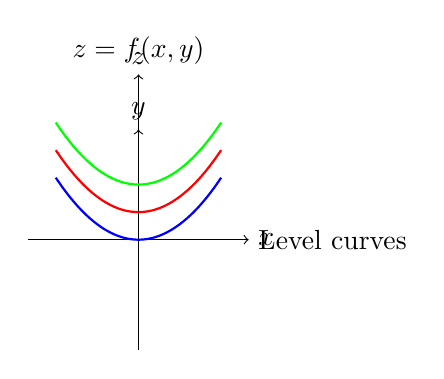
\begin{tikzpicture}[scale=0.7]
\draw[->] (-2,0) -- (2,0) node[right] {$x$};
\draw[->] (0,-2) -- (0,2) node[above] {$y$};
\draw[->] (0,0) -- (0,3) node[above] {$z$};
\draw[domain=-1.5:1.5, smooth, variable=\x, blue, thick] plot ({\x}, {0.5*\x*\x});
\draw[domain=-1.5:1.5, smooth, variable=\x, red, thick] plot ({\x}, {0.5*\x*\x + 0.5});
\draw[domain=-1.5:1.5, smooth, variable=\x, green, thick] plot ({\x}, {0.5*\x*\x + 1});
\node[above] at (0,3) {$z = f(x,y)$};
\node[right] at (2,0) {Level curves};
\end{tikzpicture}
\end{center}

\textbf{Visualization Methods:}
\begin{itemize}
    \item \textbf{3D surfaces:} Plot $z = f(x,y)$ in 3D space
    \item \textbf{Level curves:} Curves where $f(x,y) = c$ (constant)
    \item \textbf{Contour plots:} 2D representation of level curves
    \item \textbf{Cross-sections:} Fix one variable and plot the result
\end{itemize}
\end{frame}

\section{Partial Derivatives}

\begin{frame}{What are Partial Derivatives?}
\textbf{Definition:} Rate of change of a function with respect to one variable while holding others constant

\textbf{Notation:}
\begin{itemize}
    \item $\frac{\partial f}{\partial x}$ or $f_x$: partial derivative with respect to $x$
    \item $\frac{\partial f}{\partial y}$ or $f_y$: partial derivative with respect to $y$
    \item $\frac{\partial f}{\partial z}$ or $f_z$: partial derivative with respect to $z$
\end{itemize}

\textbf{Geometric Interpretation:}
\begin{itemize}
    \item $\frac{\partial f}{\partial x}$: slope of tangent line in $x$-direction
    \item $\frac{\partial f}{\partial y}$: slope of tangent line in $y$-direction
    \item Each partial derivative gives the rate of change along one axis
\end{itemize}
\end{frame}

\begin{frame}{Computing Partial Derivatives - Method}
\textbf{Method:} Treat all other variables as constants and differentiate with respect to the variable of interest

\textbf{Key Rules:}
\begin{itemize}
    \item When differentiating with respect to $x$, treat $y$ and $z$ as constants
    \item When differentiating with respect to $y$, treat $x$ and $z$ as constants
    \item Use all standard differentiation rules (product rule, chain rule, etc.)
    \item The order of partial differentiation matters for mixed partials
\end{itemize}

\textbf{Example:} For $f(x,y) = x^2 + 3xy + y^2$
\begin{align*}
    \frac{\partial f}{\partial x} &= 2x + 3y \quad \text{(treat $y$ as constant)} \\
    \frac{\partial f}{\partial y} &= 3x + 2y \quad \text{(treat $x$ as constant)}
\end{align*}
\end{frame}

\begin{frame}{Partial Derivatives - Example 1}
\textbf{Example:} $f(x,y) = e^{xy} \sin(x)$

\textbf{Solution:}
\begin{align*}
    \frac{\partial f}{\partial x} &= ye^{xy} \sin(x) + e^{xy} \cos(x) \\
    &= e^{xy}(y\sin(x) + \cos(x))
\end{align*}

\begin{align*}
    \frac{\partial f}{\partial y} &= xe^{xy} \sin(x)
\end{align*}

\textbf{Explanation:}
\begin{itemize}
    \item For $\frac{\partial f}{\partial x}$: Use product rule on $e^{xy} \sin(x)$
    \item For $\frac{\partial f}{\partial y}$: Only $e^{xy}$ depends on $y$, so $\sin(x)$ is constant
\end{itemize}
\end{frame}

\begin{frame}{Partial Derivatives - Example 2}
\textbf{Example:} $f(x,y,z) = x^2y + yz^2 + xz$

\textbf{Solution:}
\begin{align*}
    \frac{\partial f}{\partial x} &= 2xy + z \\
    \frac{\partial f}{\partial y} &= x^2 + z^2 \\
    \frac{\partial f}{\partial z} &= 2yz + x
\end{align*}

\textbf{Explanation:}
\begin{itemize}
    \item $\frac{\partial f}{\partial x}$: $x^2y$ gives $2xy$, $yz^2$ gives $0$, $xz$ gives $z$
    \item $\frac{\partial f}{\partial y}$: $x^2y$ gives $x^2$, $yz^2$ gives $z^2$, $xz$ gives $0$
    \item $\frac{\partial f}{\partial z}$: $x^2y$ gives $0$, $yz^2$ gives $2yz$, $xz$ gives $x$
\end{itemize}
\end{frame}

\begin{frame}{Partial Derivatives - Example 3}
\textbf{Example:} $f(x,y) = \frac{x^2 + y^2}{x + y}$

\textbf{Solution for $\frac{\partial f}{\partial x}$:}
\begin{align*}
    \frac{\partial f}{\partial x} &= \frac{(2x)(x + y) - (x^2 + y^2)(1)}{(x + y)^2} \\
    &= \frac{2x^2 + 2xy - x^2 - y^2}{(x + y)^2} \\
    &= \frac{x^2 + 2xy - y^2}{(x + y)^2}
\end{align*}

\textbf{Explanation:}
\begin{itemize}
    \item Used quotient rule: $\frac{d}{dx}\left[\frac{u}{v}\right] = \frac{v \cdot u' - u \cdot v'}{v^2}$
    \item $u = x^2 + y^2$, so $u' = 2x$
    \item $v = x + y$, so $v' = 1$
\end{itemize}
\end{frame}

\begin{frame}{Partial Derivatives - Example 3 (Continued)}
\textbf{Solution for $\frac{\partial f}{\partial y}$:}
\begin{align*}
    \frac{\partial f}{\partial y} &= \frac{(2y)(x + y) - (x^2 + y^2)(1)}{(x + y)^2} \\
    &= \frac{2xy + 2y^2 - x^2 - y^2}{(x + y)^2} \\
    &= \frac{2xy + y^2 - x^2}{(x + y)^2}
\end{align*}

\textbf{Explanation:}
\begin{itemize}
    \item Used quotient rule again
    \item $u = x^2 + y^2$, so $u' = 2y$ (treating $x$ as constant)
    \item $v = x + y$, so $v' = 1$
    \item Notice the symmetry between the two partial derivatives
\end{itemize}
\end{frame}

\begin{frame}{Partial Derivatives - Example 4}
\textbf{Example:} $f(x,y) = \ln(x^2 + y^2)$

\textbf{Solution:}
\begin{align*}
    \frac{\partial f}{\partial x} &= \frac{2x}{x^2 + y^2} \\
    \frac{\partial f}{\partial y} &= \frac{2y}{x^2 + y^2}
\end{align*}

\textbf{Explanation:}
\begin{itemize}
    \item Use chain rule: $\frac{d}{dx}[\ln(u)] = \frac{1}{u} \cdot \frac{du}{dx}$
    \item For $\frac{\partial f}{\partial x}$: $u = x^2 + y^2$, so $\frac{du}{dx} = 2x$
    \item For $\frac{\partial f}{\partial y}$: $u = x^2 + y^2$, so $\frac{du}{dy} = 2y$
\end{itemize}
\end{frame}

\begin{frame}{Geometric Interpretation of Partial Derivatives}
\begin{center}
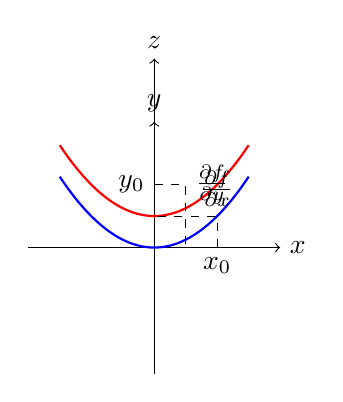
\begin{tikzpicture}[scale=0.8]
\draw[->] (-2,0) -- (2,0) node[right] {$x$};
\draw[->] (0,-2) -- (0,2) node[above] {$y$};
\draw[->] (0,0) -- (0,3) node[above] {$z$};
\draw[domain=-1.5:1.5, smooth, variable=\x, blue, thick] plot ({\x}, {0.5*\x*\x});
\draw[domain=-1.5:1.5, smooth, variable=\x, red, thick] plot ({\x}, {0.5*\x*\x + 0.5});
\draw[dashed] (1,0) -- (1,0.5) -- (0,0.5);
\draw[dashed] (0,1) -- (0.5,1) -- (0.5,0);
\node[below] at (1,0) {$x_0$};
\node[left] at (0,1) {$y_0$};
\node[above] at (1,0.5) {$\frac{\partial f}{\partial x}$};
\node[right] at (0.5,1) {$\frac{\partial f}{\partial y}$};
\end{tikzpicture}
\end{center}

\textbf{Key Points:}
\begin{itemize}
    \item $\frac{\partial f}{\partial x}$: slope of tangent line parallel to $x$-axis
    \item $\frac{\partial f}{\partial y}$: slope of tangent line parallel to $y$-axis
    \item Both partials exist at a point if the function is differentiable there
    \item Partial derivatives can exist even if the function is not continuous
\end{itemize}
\end{frame}

\section{Second Order Partial Derivatives}

\begin{frame}{Second Order Partial Derivatives - Introduction}
\textbf{Definition:} Partial derivatives of partial derivatives

\textbf{Notation:}
\begin{itemize}
    \item $\frac{\partial^2 f}{\partial x^2}$ or $f_{xx}$: second partial with respect to $x$
    \item $\frac{\partial^2 f}{\partial y^2}$ or $f_{yy}$: second partial with respect to $y$
    \item $\frac{\partial^2 f}{\partial x \partial y}$ or $f_{xy}$: mixed partial (first $x$, then $y$)
    \item $\frac{\partial^2 f}{\partial y \partial x}$ or $f_{yx}$: mixed partial (first $y$, then $x$)
\end{itemize}

\textbf{Clairaut's Theorem:} If $f_{xy}$ and $f_{yx}$ are continuous, then $f_{xy} = f_{yx}$

\textbf{Example:} For $f(x,y) = x^2y + xy^2$
\begin{align*}
    f_x &= 2xy + y^2 \\
    f_y &= x^2 + 2xy
\end{align*}
\end{frame}

\begin{frame}{Second Order Partial Derivatives - Example 1}
\textbf{Example:} $f(x,y) = x^2y + xy^2$

\textbf{First order partials:}
\begin{align*}
    f_x &= 2xy + y^2 \\
    f_y &= x^2 + 2xy
\end{align*}

\textbf{Second order partials:}
\begin{align*}
    f_{xx} &= 2y \\
    f_{yy} &= 2x \\
    f_{xy} &= 2x + 2y \\
    f_{yx} &= 2x + 2y
\end{align*}

\textbf{Note:} $f_{xy} = f_{yx}$ as expected by Clairaut's theorem.
\end{frame}

\begin{frame}{Second Order Partial Derivatives - Example 2}
\textbf{Example:} $f(x,y) = e^{xy} + x^2y$

\textbf{First order partials:}
\begin{align*}
    f_x &= ye^{xy} + 2xy \\
    f_y &= xe^{xy} + x^2
\end{align*}

\textbf{Second order partials:}
\begin{align*}
    f_{xx} &= y^2e^{xy} + 2y \\
    f_{yy} &= x^2e^{xy} \\
    f_{xy} &= e^{xy} + xye^{xy} + 2x \\
    f_{yx} &= e^{xy} + xye^{xy} + 2x
\end{align*}

\textbf{Note:} $f_{xy} = f_{yx}$ as expected.
\end{frame}

\begin{frame}{Second Order Partial Derivatives - Example 3}
\textbf{Example:} $f(x,y) = \sin(xy) + x^3y^2$

\textbf{First order partials:}
\begin{align*}
    f_x &= y\cos(xy) + 3x^2y^2 \\
    f_y &= x\cos(xy) + 2x^3y
\end{align*}

\textbf{Second order partials:}
\begin{align*}
    f_{xx} &= -y^2\sin(xy) + 6xy^2 \\
    f_{yy} &= -x^2\sin(xy) + 2x^3 \\
    f_{xy} &= \cos(xy) - xy\sin(xy) + 6x^2y \\
    f_{yx} &= \cos(xy) - xy\sin(xy) + 6x^2y
\end{align*}

\textbf{Note:} $f_{xy} = f_{yx}$ as expected.
\end{frame}

\begin{frame}{The Hessian Matrix - Introduction}
\textbf{Definition:} Matrix of second order partial derivatives

For $f(x,y)$:
\[H = \begin{bmatrix} 
f_{xx} & f_{xy} \\
f_{yx} & f_{yy}
\end{bmatrix} = \begin{bmatrix} 
\frac{\partial^2 f}{\partial x^2} & \frac{\partial^2 f}{\partial x \partial y} \\
\frac{\partial^2 f}{\partial y \partial x} & \frac{\partial^2 f}{\partial y^2}
\end{bmatrix}\]

\textbf{Properties:}
\begin{itemize}
    \item Symmetric matrix (if Clairaut's theorem applies)
    \item Used to classify critical points
    \item Determinant helps determine nature of extrema
    \item Important in optimization problems
\end{itemize}
\end{frame}

\begin{frame}{The Hessian Matrix - Example}
\textbf{Example:} For $f(x,y) = x^2 + 3xy + y^2$

\textbf{First order partials:}
\begin{align*}
    f_x &= 2x + 3y \\
    f_y &= 3x + 2y
\end{align*}

\textbf{Second order partials:}
\begin{align*}
    f_{xx} &= 2 \\
    f_{yy} &= 2 \\
    f_{xy} &= f_{yx} = 3
\end{align*}

\textbf{Hessian matrix:}
\[H = \begin{bmatrix} 
2 & 3 \\
3 & 2
\end{bmatrix}\]

\textbf{Determinant:}
\[\det(H) = (2)(2) - (3)(3) = 4 - 9 = -5\]
\end{frame}

\begin{frame}{The Hessian Matrix - Applications}
\textbf{Applications:}
\begin{itemize}
    \item \textbf{Classifying critical points:}
    \begin{itemize}
        \item If $\det(H) > 0$ and $f_{xx} > 0$: local minimum
        \item If $\det(H) > 0$ and $f_{xx} < 0$: local maximum
        \item If $\det(H) < 0$: saddle point
        \item If $\det(H) = 0$: inconclusive (degenerate case)
    \end{itemize}
    \item \textbf{Optimization problems:} Finding extrema of functions
    \item \textbf{Taylor series expansions:} Second order approximation
    \item \textbf{Convexity/concavity:} Determining function behavior
\end{itemize}
\end{frame}

\section{Practice Problems}

\begin{frame}{Practice Problem 1}
\textbf{Problem:} Find all first and second order partial derivatives of $f(x,y) = x^3y^2 + e^{xy}$

\textbf{Steps to follow:}
\begin{enumerate}
    \item Find $f_x$ and $f_y$ (first order partials)
    \item Find $f_{xx}$, $f_{yy}$, $f_{xy}$, and $f_{yx}$ (second order partials)
    \item Verify that $f_{xy} = f_{yx}$ (Clairaut's theorem)
\end{enumerate}

\textbf{Hint:} Remember to use the product rule and chain rule where needed.
\end{frame}

\begin{frame}{Practice Problem 2}
\textbf{Problem:} Find all first and second order partial derivatives of $f(x,y) = \ln(x^2 + y^2)$

\textbf{Steps to follow:}
\begin{enumerate}
    \item Find $f_x$ and $f_y$ using the chain rule
    \item Find $f_{xx}$, $f_{yy}$, $f_{xy}$, and $f_{yx}$
    \item Simplify your answers
\end{enumerate}

\textbf{Hint:} For the second derivatives, you'll need to use the quotient rule.
\end{frame}

\begin{frame}{Practice Problem 3}
\textbf{Problem:} Find all first and second order partial derivatives of $f(x,y,z) = x^2y + yz^2 + xz$

\textbf{Steps to follow:}
\begin{enumerate}
    \item Find $f_x$, $f_y$, and $f_z$ (first order partials)
    \item Find all second order partials: $f_{xx}$, $f_{yy}$, $f_{zz}$, $f_{xy}$, $f_{xz}$, $f_{yx}$, $f_{yz}$, $f_{zx}$, $f_{zy}$
    \item Verify that mixed partials are equal where applicable
\end{enumerate}

\textbf{Hint:} This is a relatively simple function - each term depends on at most two variables.
\end{frame}

\begin{frame}{Practice Problem 4}
\textbf{Problem:} Find the Hessian matrix for $f(x,y) = x^2 + 2xy + y^2$

\textbf{Steps to follow:}
\begin{enumerate}
    \item Find all second order partial derivatives
    \item Construct the Hessian matrix
    \item Calculate the determinant of the Hessian
\end{enumerate}

\textbf{Hint:} This is a quadratic function, so the second derivatives will be constants.
\end{frame}

\begin{frame}{Practice Problem 5}
\textbf{Problem:} Show that $f(x,y) = \frac{x^2 - y^2}{x^2 + y^2}$ satisfies the equation $xf_x + yf_y = 0$

\textbf{Steps to follow:}
\begin{enumerate}
    \item Find $f_x$ and $f_y$ using the quotient rule
    \item Compute $xf_x + yf_y$
    \item Simplify to show it equals zero
\end{enumerate}

\textbf{Hint:} This is a homogeneous function of degree 0, which explains why this equation holds.
\end{frame}

\begin{frame}{Practice Problem 6}
\textbf{Problem:} Find all first and second order partial derivatives of $f(x,y) = \sin(xy) + \cos(x + y)$

\textbf{Steps to follow:}
\begin{enumerate}
    \item Find $f_x$ and $f_y$ using trigonometric differentiation rules
    \item Find all second order partials
    \item Verify Clairaut's theorem
\end{enumerate}

\textbf{Hint:} Remember that $\frac{d}{dx}[\sin(u)] = \cos(u) \cdot \frac{du}{dx}$ and $\frac{d}{dx}[\cos(u)] = -\sin(u) \cdot \frac{du}{dx}$.
\end{frame}

\begin{frame}{Practice Problem 7}
\textbf{Problem:} Find all first and second order partial derivatives of $f(x,y) = e^{x^2 + y^2}$

\textbf{Steps to follow:}
\begin{enumerate}
    \item Find $f_x$ and $f_y$ using the chain rule
    \item Find all second order partials
    \item Verify Clairaut's theorem
\end{enumerate}

\textbf{Hint:} This is a radial function, so it has special symmetry properties.
\end{frame}

\begin{frame}{Practice Problem 8}
\textbf{Problem:} Find the Hessian matrix for $f(x,y) = x^3 + y^3 - 3xy$

\textbf{Steps to follow:}
\begin{enumerate}
    \item Find all first and second order partial derivatives
    \item Construct the Hessian matrix
    \item Calculate the determinant
    \item What does this tell you about the critical points?
\end{enumerate}

\textbf{Hint:} This function has interesting critical point behavior.
\end{frame}

\section{Solutions to Practice Problems}

\begin{frame}{Practice Problem 1 - Solution}
\textbf{Solution:} $f(x,y) = x^3y^2 + e^{xy}$

\textbf{First order partials:}
\begin{align*}
    f_x &= 3x^2y^2 + ye^{xy} \\
    f_y &= 2x^3y + xe^{xy}
\end{align*}

\textbf{Second order partials:}
\begin{align*}
    f_{xx} &= 6xy^2 + y^2e^{xy} \\
    f_{yy} &= 2x^3 + x^2e^{xy} \\
    f_{xy} &= 6x^2y + e^{xy} + xye^{xy} \\
    f_{yx} &= 6x^2y + e^{xy} + xye^{xy}
\end{align*}

\textbf{Note:} $f_{xy} = f_{yx}$ as expected by Clairaut's theorem.
\end{frame}

\begin{frame}{Practice Problem 2 - Solution}
\textbf{Solution:} $f(x,y) = \ln(x^2 + y^2)$

\textbf{First order partials:}
\begin{align*}
    f_x &= \frac{2x}{x^2 + y^2} \\
    f_y &= \frac{2y}{x^2 + y^2}
\end{align*}

\textbf{Second order partials:}
\begin{align*}
    f_{xx} &= \frac{2(x^2 + y^2) - 2x(2x)}{(x^2 + y^2)^2} = \frac{2y^2 - 2x^2}{(x^2 + y^2)^2} \\
    f_{yy} &= \frac{2(x^2 + y^2) - 2y(2y)}{(x^2 + y^2)^2} = \frac{2x^2 - 2y^2}{(x^2 + y^2)^2}
\end{align*}
\end{frame}

\begin{frame}{Practice Problem 2 - Solution (Continued)}
\textbf{Second order partials (continued):}
\begin{align*}
    f_{xy} &= \frac{-2x(2y)}{(x^2 + y^2)^2} = \frac{-4xy}{(x^2 + y^2)^2} \\
    f_{yx} &= \frac{-2y(2x)}{(x^2 + y^2)^2} = \frac{-4xy}{(x^2 + y^2)^2}
\end{align*}

\textbf{Note:} $f_{xy} = f_{yx}$ and $f_{xx} = -f_{yy}$.

\textbf{Explanation:}
\begin{itemize}
    \item Used quotient rule for second derivatives
    \item Mixed partials are equal as expected by Clairaut's theorem
    \item Pure second derivatives have opposite signs due to symmetry
\end{itemize}
\end{frame}

\begin{frame}{Practice Problem 3 - Solution}
\textbf{Solution:} $f(x,y,z) = x^2y + yz^2 + xz$

\textbf{First order partials:}
\begin{align*}
    f_x &= 2xy + z \\
    f_y &= x^2 + z^2 \\
    f_z &= 2yz + x
\end{align*}

\textbf{Explanation:}
\begin{itemize}
    \item $\frac{\partial f}{\partial x}$: $x^2y$ gives $2xy$, $yz^2$ gives $0$, $xz$ gives $z$
    \item $\frac{\partial f}{\partial y}$: $x^2y$ gives $x^2$, $yz^2$ gives $z^2$, $xz$ gives $0$
    \item $\frac{\partial f}{\partial z}$: $x^2y$ gives $0$, $yz^2$ gives $2yz$, $xz$ gives $x$
\end{itemize}
\end{frame}

\begin{frame}{Practice Problem 3 - Solution (Continued)}
\textbf{Second order partials:}
\begin{align*}
    f_{xx} &= 2y \\
    f_{yy} &= 0 \\
    f_{zz} &= 2y
\end{align*}

\textbf{Mixed partials:}
\begin{align*}
    f_{xy} &= 2x = f_{yx} \\
    f_{xz} &= 1 = f_{zx} \\
    f_{yz} &= 2z = f_{zy}
\end{align*}

\textbf{Note:} All mixed partials are equal as expected by Clairaut's theorem.

\textbf{Key observations:}
\begin{itemize}
    \item Pure second derivatives with respect to $x$ and $z$ are equal ($f_{xx} = f_{zz} = 2y$)
    \item Pure second derivative with respect to $y$ is zero ($f_{yy} = 0$)
    \item All mixed partials are constants
\end{itemize}
\end{frame}

\begin{frame}{Practice Problem 4 - Solution}
\textbf{Solution:} $f(x,y) = x^2 + 2xy + y^2$

\textbf{Second order partials:}
\begin{align*}
    f_{xx} &= 2 \\
    f_{yy} &= 2 \\
    f_{xy} &= 2 = f_{yx}
\end{align*}

\textbf{Hessian matrix:}
\[H = \begin{bmatrix} 
2 & 2 \\
2 & 2
\end{bmatrix}\]

\textbf{Determinant:}
\[\det(H) = (2)(2) - (2)(2) = 4 - 4 = 0\]

\textbf{Interpretation:} This indicates that the function has a degenerate critical point structure.
\end{frame}

\begin{frame}{Practice Problem 5 - Solution}
\textbf{Solution:} $f(x,y) = \frac{x^2 - y^2}{x^2 + y^2}$

\textbf{First order partial - $\frac{\partial f}{\partial x}$:}
\begin{align*}
    f_x &= \frac{(2x)(x^2 + y^2) - (x^2 - y^2)(2x)}{(x^2 + y^2)^2} \\
    &= \frac{2x^3 + 2xy^2 - 2x^3 + 2xy^2}{(x^2 + y^2)^2} \\
    &= \frac{4xy^2}{(x^2 + y^2)^2}
\end{align*}

\textbf{Explanation:}
\begin{itemize}
    \item Used quotient rule: $\frac{d}{dx}\left[\frac{u}{v}\right] = \frac{v \cdot u' - u \cdot v'}{v^2}$
    \item $u = x^2 - y^2$, so $u' = 2x$
    \item $v = x^2 + y^2$, so $v' = 2x$
    \item Notice the cancellation: $2x^3 - 2x^3 = 0$
\end{itemize}
\end{frame}

\begin{frame}{Practice Problem 5 - Solution (Continued)}
\textbf{First order partial - $\frac{\partial f}{\partial y}$:}
\begin{align*}
    f_y &= \frac{(-2y)(x^2 + y^2) - (x^2 - y^2)(2y)}{(x^2 + y^2)^2} \\
    &= \frac{-2x^2y - 2y^3 - 2x^2y + 2y^3}{(x^2 + y^2)^2} \\
    &= \frac{-4x^2y}{(x^2 + y^2)^2}
\end{align*}

\textbf{Explanation:}
\begin{itemize}
    \item Used quotient rule again
    \item $u = x^2 - y^2$, so $u' = -2y$
    \item $v = x^2 + y^2$, so $v' = 2y$
    \item Notice the cancellation: $-2y^3 + 2y^3 = 0$
\end{itemize}
\end{frame}

\begin{frame}{Practice Problem 5 - Solution (Verification)}
\textbf{Verification:} Show that $xf_x + yf_y = 0$

\begin{align*}
    xf_x + yf_y &= x \cdot \frac{4xy^2}{(x^2 + y^2)^2} + y \cdot \frac{-4x^2y}{(x^2 + y^2)^2} \\
    &= \frac{4x^2y^2 - 4x^2y^2}{(x^2 + y^2)^2} = 0
\end{align*}

\textbf{Explanation:} This function is homogeneous of degree 0, meaning $f(tx, ty) = f(x,y)$ for all $t \neq 0$. 

\textbf{Euler's theorem} for homogeneous functions states that $xf_x + yf_y = nf(x,y)$ where $n$ is the degree. Since $n = 0$, we get $xf_x + yf_y = 0$.

\textbf{Physical interpretation:} This function represents the ratio of the difference to the sum of squares, which has rotational symmetry.
\end{frame}

\begin{frame}{Practice Problem 6 - Solution}
\textbf{Solution:} $f(x,y) = \sin(xy) + \cos(x + y)$

\textbf{First order partials:}
\begin{align*}
    f_x &= y\cos(xy) - \sin(x + y) \\
    f_y &= x\cos(xy) - \sin(x + y)
\end{align*}

\textbf{Second order partials:}
\begin{align*}
    f_{xx} &= -y^2\sin(xy) - \cos(x + y) \\
    f_{yy} &= -x^2\sin(xy) - \cos(x + y) \\
    f_{xy} &= \cos(xy) - xy\sin(xy) - \cos(x + y) \\
    f_{yx} &= \cos(xy) - xy\sin(xy) - \cos(x + y)
\end{align*}

\textbf{Note:} $f_{xy} = f_{yx}$ as expected by Clairaut's theorem.
\end{frame}

\begin{frame}{Practice Problem 7 - Solution}
\textbf{Solution:} $f(x,y) = e^{x^2 + y^2}$

\textbf{First order partials:}
\begin{align*}
    f_x &= 2xe^{x^2 + y^2} \\
    f_y &= 2ye^{x^2 + y^2}
\end{align*}

\textbf{Second order partials:}
\begin{align*}
    f_{xx} &= 2e^{x^2 + y^2} + 4x^2e^{x^2 + y^2} = 2e^{x^2 + y^2}(1 + 2x^2) \\
    f_{yy} &= 2e^{x^2 + y^2} + 4y^2e^{x^2 + y^2} = 2e^{x^2 + y^2}(1 + 2y^2) \\
    f_{xy} &= 4xye^{x^2 + y^2} = f_{yx}
\end{align*}

\textbf{Note:} This is a radial function, so it has special symmetry properties.
\end{frame}

\begin{frame}{Practice Problem 8 - Solution}
\textbf{Solution:} $f(x,y) = x^3 + y^3 - 3xy$

\textbf{First order partials:}
\begin{align*}
    f_x &= 3x^2 - 3y \\
    f_y &= 3y^2 - 3x
\end{align*}

\textbf{Second order partials:}
\begin{align*}
    f_{xx} &= 6x \\
    f_{yy} &= 6y \\
    f_{xy} &= -3 = f_{yx}
\end{align*}

\textbf{Hessian matrix:}
\[H = \begin{bmatrix} 
6x & -3 \\
-3 & 6y
\end{bmatrix}\]

\textbf{Determinant:}
\[\det(H) = (6x)(6y) - (-3)(-3) = 36xy - 9\]
\end{frame}

\begin{frame}{Practice Problem 8 - Solution (Continued)}
\textbf{Critical points:} Set $f_x = 0$ and $f_y = 0$
\begin{align*}
    3x^2 - 3y &= 0 \quad \Rightarrow \quad y = x^2 \\
    3y^2 - 3x &= 0 \quad \Rightarrow \quad x = y^2
\end{align*}

Substituting: $x = (x^2)^2 = x^4$, so $x(x^3 - 1) = 0$

This gives $x = 0$ or $x = 1$

\textbf{Critical points:} $(0,0)$ and $(1,1)$

\textbf{At $(0,0)$:} $\det(H) = 36(0)(0) - 9 = -9 < 0$ (saddle point)

\textbf{At $(1,1)$:} $\det(H) = 36(1)(1) - 9 = 27 > 0$ and $f_{xx} = 6 > 0$ (local minimum)
\end{frame}

\section{Applications and Extensions}

\begin{frame}{Applications of Partial Derivatives - Physics}
\textbf{Physics Applications:}
\begin{itemize}
    \item \textbf{Temperature gradients:} $\nabla T = \left(\frac{\partial T}{\partial x}, \frac{\partial T}{\partial y}, \frac{\partial T}{\partial z}\right)$
    \item \textbf{Force fields:} $\vec{F} = \nabla \phi$ (gradient of potential)
    \item \textbf{Wave equations:} $\frac{\partial^2 u}{\partial t^2} = c^2\nabla^2 u$
    \item \textbf{Heat equation:} $\frac{\partial u}{\partial t} = \alpha \nabla^2 u$
    \item \textbf{Maxwell's equations:} Electromagnetic field theory
\end{itemize}

\textbf{Examples:}
\begin{itemize}
    \item Temperature distribution in a room: $T(x,y,z,t)$
    \item Electric potential: $V(x,y,z)$
    \item Wave propagation: $u(x,y,z,t)$
\end{itemize}
\end{frame}

\begin{frame}{Applications of Partial Derivatives - Economics}
\textbf{Economics Applications:}
\begin{itemize}
    \item \textbf{Marginal products:} $\frac{\partial Q}{\partial L}$ (marginal product of labor)
    \item \textbf{Elasticity:} $\frac{\partial Q}{\partial P} \cdot \frac{P}{Q}$
    \item \textbf{Utility functions:} $\frac{\partial U}{\partial x_i}$ (marginal utility)
    \item \textbf{Cost functions:} $\frac{\partial C}{\partial q_i}$ (marginal cost)
    \item \textbf{Production functions:} $Q = f(K,L)$ (output as function of capital and labor)
\end{itemize}

\textbf{Examples:}
\begin{itemize}
    \item Cobb-Douglas production: $Q = AK^\alpha L^\beta$
    \item Utility maximization: $U(x,y) = x^a y^b$
    \item Cost minimization: $C(x,y) = px + qy$
\end{itemize}
\end{frame}

\begin{frame}{Applications of Partial Derivatives - Engineering}
\textbf{Engineering Applications:}
\begin{itemize}
    \item \textbf{Stress analysis:} Second derivatives in elasticity
    \item \textbf{Fluid dynamics:} Navier-Stokes equations
    \item \textbf{Heat transfer:} Fourier's law
    \item \textbf{Structural analysis:} Beam deflection equations
    \item \textbf{Control systems:} State space representation
\end{itemize}

\textbf{Examples:}
\begin{itemize}
    \item Heat conduction: $\frac{\partial T}{\partial t} = \alpha \nabla^2 T$
    \item Beam bending: $\frac{\partial^2 w}{\partial x^2} = \frac{M}{EI}$
    \item Fluid flow: $\frac{\partial \vec{v}}{\partial t} + (\vec{v} \cdot \nabla)\vec{v} = -\frac{1}{\rho}\nabla p$
\end{itemize}
\end{frame}

\begin{frame}{The Gradient Vector - Introduction}
\textbf{Definition:} Vector of first order partial derivatives

For $f(x,y)$: $\nabla f = \left(\frac{\partial f}{\partial x}, \frac{\partial f}{\partial y}\right)$

For $f(x,y,z)$: $\nabla f = \left(\frac{\partial f}{\partial x}, \frac{\partial f}{\partial y}, \frac{\partial f}{\partial z}\right)$

\textbf{Properties:}
\begin{itemize}
    \item Points in direction of steepest increase
    \item Magnitude gives rate of steepest increase
    \item Perpendicular to level curves/surfaces
    \item Used in optimization algorithms
\end{itemize}
\end{frame}

\begin{frame}{The Gradient Vector - Examples}
\textbf{Example 1:} For $f(x,y) = x^2 + y^2$
\[\nabla f = (2x, 2y)\]

At point $(1,2)$: $\nabla f = (2, 4)$

\textbf{Example 2:} For $f(x,y) = e^{xy}$
\[\nabla f = (ye^{xy}, xe^{xy})\]

At point $(0,1)$: $\nabla f = (e^0, 0) = (1, 0)$

\textbf{Example 3:} For $f(x,y,z) = x^2 + y^2 + z^2$
\[\nabla f = (2x, 2y, 2z)\]

At point $(1,1,1)$: $\nabla f = (2, 2, 2)$
\end{frame}

\begin{frame}{The Laplacian Operator - Introduction}
\textbf{Definition:} Sum of second order partial derivatives

For $f(x,y)$: $\nabla^2 f = \frac{\partial^2 f}{\partial x^2} + \frac{\partial^2 f}{\partial y^2}$

For $f(x,y,z)$: $\nabla^2 f = \frac{\partial^2 f}{\partial x^2} + \frac{\partial^2 f}{\partial y^2} + \frac{\partial^2 f}{\partial z^2}$

\textbf{Physical Interpretation:}
\begin{itemize}
    \item Measures the "curvature" of a function
    \item Positive Laplacian: function is "concave up" in all directions
    \item Negative Laplacian: function is "concave down" in all directions
    \item Zero Laplacian: harmonic function (important in physics)
\end{itemize}
\end{frame}

\begin{frame}{The Laplacian Operator - Applications}
\textbf{Applications:}
\begin{itemize}
    \item \textbf{Heat equation:} $\frac{\partial u}{\partial t} = \alpha \nabla^2 u$
    \item \textbf{Wave equation:} $\frac{\partial^2 u}{\partial t^2} = c^2 \nabla^2 u$
    \item \textbf{Poisson's equation:} $\nabla^2 \phi = \rho$
    \item \textbf{Laplace's equation:} $\nabla^2 \phi = 0$
    \item \textbf{Schrödinger equation:} $i\hbar\frac{\partial \psi}{\partial t} = -\frac{\hbar^2}{2m}\nabla^2 \psi + V\psi$
\end{itemize}

\textbf{Examples:}
\begin{itemize}
    \item For $f(x,y) = x^2 + y^2$: $\nabla^2 f = 2 + 2 = 4$
    \item For $f(x,y) = \sin(x)\cos(y)$: $\nabla^2 f = -\sin(x)\cos(y) - \sin(x)\cos(y) = -2\sin(x)\cos(y)$
    \item For $f(x,y) = \ln(x^2 + y^2)$: $\nabla^2 f = 0$ (harmonic function)
\end{itemize}
\end{frame}

\begin{frame}{Summary - Key Concepts}
\begin{itemize}
    \item \textbf{Multivariable functions} depend on multiple variables
    \item \textbf{Partial derivatives} measure rate of change with respect to one variable
    \item \textbf{Second order partials} include pure and mixed derivatives
    \item \textbf{Clairaut's theorem} states that mixed partials are equal under continuity
    \item \textbf{Hessian matrix} organizes second order partials
    \item \textbf{Gradient vector} points in direction of steepest increase
    \item \textbf{Laplacian operator} is sum of pure second order partials
\end{itemize}
\end{frame}

\begin{frame}{Summary - Applications}
\begin{itemize}
    \item \textbf{Physics:} Temperature gradients, force fields, wave equations
    \item \textbf{Economics:} Marginal products, elasticity, utility functions
    \item \textbf{Engineering:} Stress analysis, fluid dynamics, heat transfer
    \item \textbf{Optimization:} Finding extrema, gradient descent algorithms
    \item \textbf{Computer Science:} Machine learning, computer graphics
    \item \textbf{Biology:} Population dynamics, diffusion processes
\end{itemize}
\end{frame}

\begin{frame}{Thank You!}
\centering
\vspace{2cm}
{\Huge \textcolor{myblue}{\textbf{Questions?}}}

\vspace{1cm}
{\Large Multivariable calculus opens the door to understanding complex systems in multiple dimensions!}

\vspace{0.5cm}
{\large \textcolor{myorange}{Next: Optimization, Lagrange multipliers, and multiple integrals}}
\end{frame}

\end{document} 